
\includegraphics[height=1.25cm]{images/pictograms/FEM}

\includegraphics[height=1.25cm]{images/pictograms/benchmark}

\begin{flushright} {\tiny {\color{gray} python\_codes/fieldstone\_01/text.tex}} \end{flushright}

\lstinputlisting[language=bash,basicstyle=\small]{python_codes/fieldstone_01/keywords.ascii}

\begin{center}
\inpython
\injulia
\infortran
{\small Codes: \url{https://github.com/cedrict/fieldstone/tree/master/python_codes/fieldstone_01}}
\end{center}

\par\noindent\rule{\textwidth}{0.4pt}

{\sl The python stone was developed in collaboration with Job Mos}. \index{contributors}{J. Mos}
{\sl The julia stone was developed by Jort Jansen.}. \index{contributors}{J. Jansen}

\par\noindent\rule{\textwidth}{0.4pt}
%%%%%%%%%%%%%%%%%%%%%%%%%%%%%%%%%%%%%%%%%%%%%%%%%%%%%%%%%%%%%%%%%%%%%%%%%%%%%%%%%%%%%%%%%%%%%%

This benchmark is taken from Donea \& Huerta (2003) \cite{dohu03} and is described fully in section \ref{MMM-mms1}. 
In order to illustrate the behavior of selected mixed finite elements in the solution 
of stationary Stokes flow,  we consider a two-dimensional problem 
in the square domain $\Omega=[0,1]\times[0,1]$, which possesses a closed-form analytical 
solution. 

\begin{center}
\includegraphics[width=10cm]{python_codes/fieldstone_01/results/errors.pdf}\\
{\captionfont Quadratic convergence for velocity error, 
linear convergence for pressure error, as expected.}
\end{center}

\begin{center}
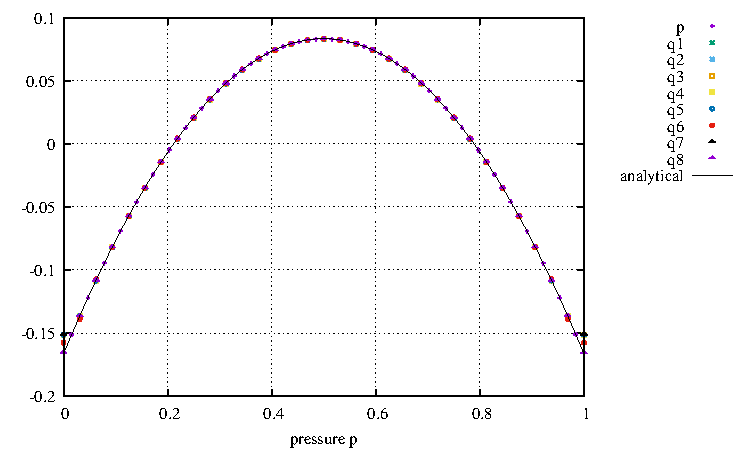
\includegraphics[width=11cm]{python_codes/fieldstone_01/results/pressure.pdf}\\
{\captionfont Pressure field}
\end{center}

\begin{center}
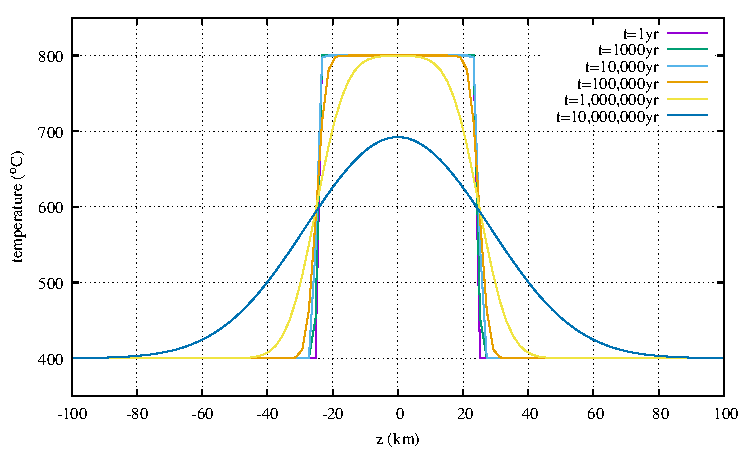
\includegraphics[width=16cm]{python_codes/fieldstone_01/results/solution.pdf}
\end{center}

One can also compute vertical/depth averages of the velocity, see Eq.~\eqref{MMM-eq:dhvelnorm}.
Note that the averages are computed somewhat naively: instead of computing integrals in the $x$-direction
at many depths I simply take an arithmetic average over rows of nodes. At high resolution the profiles
converge to the analytical profiles for the individual components and to the results 
obtained with \aspect. Please check \stone~\ref{f110} for a better implementation.
\begin{center}
\includegraphics[width=12cm]{python_codes/fieldstone_01/results/vel_profile}\\
{\captionfont Vertical average of velocity. \aspect was run with the 'depth average' postprocessor
added to the prm file.}
\end{center}

\newpage
\subsection*{About the Fortran code}

I wrote the first ever version of this \stone in
Fortran90 around 2011. It is available in the {\foldernamefont simplefem} folder in this stone.
\index{general}{fortran90}

The code can be compiled as follows:
\begin{verbatim}
> gfortran -O3 linpack_d.f90 blas_routines.f simplefem.f90
\end{verbatim}
and run as follows:
\begin{verbatim}
> ./a.out 
\end{verbatim}
The solver used here does not make use of a sparse storage and relies on a dense matrix 
set of subroutine from BLAS and LinPACK\footnote{\url{https://en.wikipedia.org/wiki/LINPACK}}.
\begin{center}
\includegraphics[width=11cm]{python_codes/fieldstone_01/simplefem/timings/timings.pdf}\\
{\captionfont Despite a very naive application of the boundary conditions to the entire
assembled FE matrix, we find here that this part of the code is not taking long at all.}
\end{center}
There is no export of the results to ParaView format, only ascii text files.



\newpage
\subsection*{About the Julia code}

The python code was translated to julia in a rather straightforward manner. 
The matrix is still a full array (no sparse storage during the build process) 
and the boundary conditions
are applied naively. Even with a $80\times 80$ resolution the memory use is under 2Gb. 
Note that there seems to be a limit as to the maximum size of the matrix array 
and for instance $96\times 96$ yields to a crash.

In this version the matrix is stored as a full array. 
Before the linear system is solved, however, we must convert it to sparse storage:
\begin{verbatim}
Sps_amat=sparse(a_mat)
\end{verbatim}
When it comes to the solve, we have various options. The first and most 
simple one is similar to Matlab's backslash:
\begin{verbatim}
sol= Sps_amat\rhs
\end{verbatim}
Another possibility is cholesky\footnote{This method uses the CHOLMOD library from SuiteSparse:
\url{https://people.engr.tamu.edu/davis/suitesparse.html}} or ldlt or lu:
\begin{verbatim}
sol= cholesky(Sps_amat)\rhs
sol= ldlt(Sps_amat)\rhs
sol= lu(Sps_amat)\rhs
\end{verbatim}


The computed errors are of course identical to those of the python codes but we find that
at low resolutions the python code is much faster than the julia code: 
this is likely due to the time taken by julia to compile the code.
 

\begin{center}
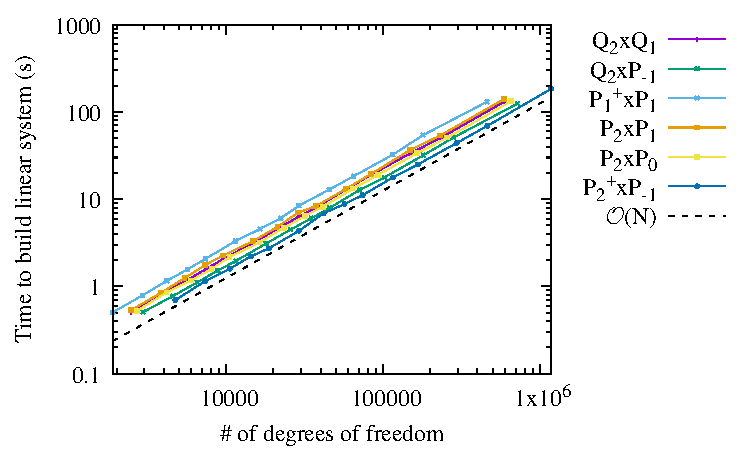
\includegraphics[width=8cm]{python_codes/fieldstone_01/results/julia/timings_build.pdf}
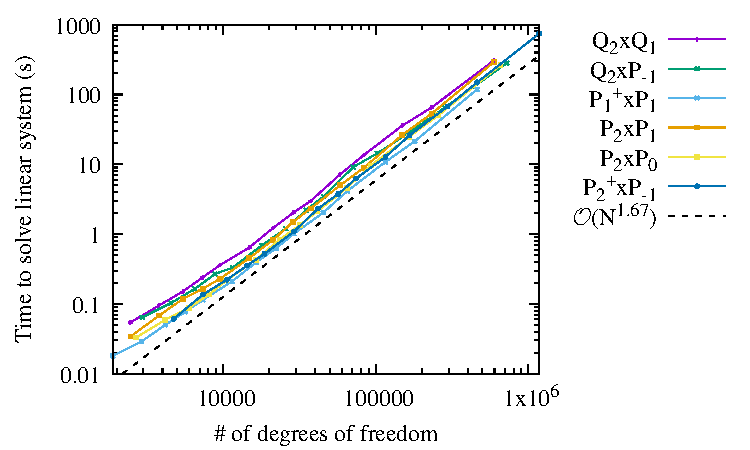
\includegraphics[width=8cm]{python_codes/fieldstone_01/results/julia/timings_solve.pdf}\\
\includegraphics[width=11cm]{python_codes/fieldstone_01/results/julia/errors.pdf}\\
{\captionfont Matrix building and solving times as obtained for nelx from 8 until 80, each 
resolution being run 10 times.}
\end{center}

We find that the LU-based solver is the fasted in this case.





